\documentclass{report}

\usepackage[utf8]{inputenc}
\usepackage[brazil]{babel}
\usepackage{mathtools}
\usepackage{graphicx}
\graphicspath{{./Imagens/}}
\usepackage{subcaption}
\usepackage{epstopdf}
\usepackage{float}
\usepackage{listings}
\usepackage{courier}
\usepackage{eqnarray}
\usepackage{amsmath}
\usepackage{amsfonts}
\usepackage[dvipsnames]{xcolor}
\usepackage{verbatim}

\lstset{
	backgroundcolor=\color[rgb]{1,1,0.9},
	frame = single,
	basicstyle = \footnotesize,
	keywordstyle = \color{blue},
	commentstyle = \color[rgb]{0,0.5,0},
	stringstyle = \color{Purple},
	showstringspaces = false,
	mathescape,
	breaklines = true,
	language = Matlab,
	inputencoding = utf8,
	extendedchars = true,
	literate = {ã}{{\~a}} 1
			   {é}{{\'e}} 1
			   {ç}{{\c{c}}} 1
			   {~}{{$\sim\ $}} 1
			   {ó}{{\'o}} 1
			   {á}{{\'a}} 1
			   {ú}{{\'u}} 1
			   {õ}{{\~o}} 1
			   {í}{{\'i}} 1
			   {Í}{{\'I}} 1
}

\begin{document}

\begin{titlepage}
\begin{flushleft}

\textsc{\textbf{\LARGE Universidade Federal do Rio de Janeiro}}\\[0.5cm]
\textsc{\textbf{\LARGE COPPE}}\\[0.5cm]
\textsc{\textbf{\LARGE Programa de Engenharia Elétrica - PEE}}\\[0.5cm]
\textsc{\textbf{\LARGE Disciplina: Otimização Natural}}\\[0.5cm]
\textsc{\textbf{\LARGE Aluno: Gustavo Martins da Silva Nunes}}\\[0.5cm]
\textsc{\textbf{\LARGE Professor: José Gabriel}}\\[0.5cm]
\textsc{\textbf{\LARGE Data: 15/03/2016}}\\[6.5cm]

\end{flushleft}
\begin{center}
\textsc{\textbf{\huge Lista 1 - Resolução}}
\vfill
\end{center}
\end{titlepage}

\section*{Questão 1}

\textbf{\textit{Capítulo 5, Exercício 7}:}\\

\textbf{Implement an EP for the Ackley function with $n = 30$. Make 100 runs, storing the best value found in each, and then calculate the mean and standard deviation of these values. Compare your results with those from exercises 5 and 6 in Chap. 4.}\\

\paragraph{} O código, feito em MATLAB, que implementa a solução da questão, encontra-se abaixo.\\

\begin{lstlisting}
clear all; close all; clc

N_pop = 200; % Tamanho da população
N_avaliacoes = 200000; % Quantidade de avaliações da função de Ackley
N_ger = N_avaliacoes/N_pop; % Número de gerações avaliadas 
n = 30; % Dimensões da função de Ackley
epsilon = 0.02; % Tamanho mínimo do passo de alteração
eta = 6; % Passo de alteração inicial
N_exec = 100; % Número de execuções do algoritmo
alpha = 0.2; % Constante de alteração do passo
q = 10; % Quantidade de vezes que uma solução participará do torneio
melhor_fitness_execucao = ones(1, N_exec); % Melhores fitness encontradas em cada execução do algoritmo
geracao_otima_execucao = zeros(1, N_exec); % Primeira geração em que apareceu a melhor fitness em cada execução do algoritmo

for t = 1:N_exec
    
    ger = 1; % Geração atual
    melhores_fitness = ones(1, N_ger); % Melhores fitness por geração 
    P = [unifrnd(-30,30,n,N_pop); eta*ones(n,N_pop)]; % Inicialização aleatória da população
    
    % Cálculo do fitness
    
    fitness = -20 * exp(-0.2 * sqrt((1/n) * sum(P(1:n,:).^2, 1))) - exp((1/n) * sum(cos(2 * pi * P(1:n,:)), 1)) + 20 + exp(1); % Fitness por indivíduos 
    
    melhores_fitness(ger) = min(fitness);
    
    while (ger <= N_ger) && (melhores_fitness(ger) > 1e-7)
        
        % Mutação
        
        P_filhos = zeros(size(P));
        
        passos = P((n+1):end, :);
        passos = passos .* (1 + alpha * (ones(n, 1) * randn(1, N_pop))); % Mutação dos passos;
        passos(passos < epsilon) = epsilon;
        
        P_filhos((n+1):end, :) = passos;
        
        P_filhos(1:n, :) = P(1:n, :) + passos .* randn(n, N_pop);
        
        % Seleção de sobreviventes
        
        P_torneio = [P P_filhos]; % Monta a população de filhos + pai para o torneio
        fitness = -20 * exp(-0.2 * sqrt((1/n) * sum(P_torneio(1:n,:).^2, 1))) - exp((1/n) * sum(cos(2 * pi * P_torneio(1:n,:)), 1)) + 20 + exp(1); % Fitness dos participantes
        resultados = zeros(1,size(P_torneio, 2)); % Resultados do torneio;
        qtd_participacoes = zeros(1,size(P_torneio, 2)); % Contagem de participações de cada indivíduo no torneio

        for p1 = 1:length(resultados)
            while (qtd_participacoes(p1) ~= q)
                
                qtd_participacoes(p1) = qtd_participacoes(p1) + 1;
                
                competidores_disponiveis = find(qtd_participacoes ~= q);                    
                p2 = unidrnd(size(P_torneio, 2));
                
                if length(competidores_disponiveis) > 1 % Há mais de um competidor disponível
                    while (p2 == p1) || (qtd_participacoes(p2) == q) % Evita sortear o mesmo participante ou um participante que já competiu o número máximo de vezes no torneio
                        p2 = unidrnd(size(P_torneio, 2));
                    end
                                        
                    qtd_participacoes(p2) = qtd_participacoes(p2) + 1;
                    
                    if fitness(p1) < fitness(p2)
                        resultados(p1) = resultados(p1) + 3;
                    else if fitness(p1) == fitness(p2)
                            resultados(p1) = resultados(p1) + 1;
                            resultados(p2) = resultados(p2) + 1;
                        else
                            resultados(p2) = resultados(p2) + 3;
                        end
                    end
                    
                else if length(competidores_disponiveis) == 1 % Sobrou somente 1 competidor; aceita sortear outro que já competiu 'q' vezes, porém não o pontua
                    while (p2 == p1) % Sorteia outro competidor, que não o próprio
                        p2 = unidrnd(size(P_torneio, 2));
                    end
                    
                    if fitness(p1) < fitness(p2)
                        resultados(p1) = resultados(p1) + 3;
                    else if fitness(p1) == fitness(p2)
                            resultados(p1) = resultados(p1) + 1;
                            resultados(p2) = resultados(p2) + 1;
                        end
                    end
                    end
                end                        
            end
        end
        
        idx = zeros(1, N_pop); % Índice que identifica os indivíduos melhor classificados
        
        for i = 1:N_pop % Salva os N_pop indivíduos melhores classificados no torneio para a próxima geração
            idx(i) = find(resultados == max(resultados), 1);
            P(:,i) = P_torneio(:,idx(i));
            resultados(idx(i)) = -Inf;
        end
        
        ger = ger + 1;
        
        fitness = fitness(idx);
        melhores_fitness(ger) = min(fitness);              
        
    end
    
    melhor_fitness_execucao(t) = min(melhores_fitness);
    geracao_otima_execucao(t) = find(melhores_fitness == min(melhores_fitness), 1);
end
\end{lstlisting}

\paragraph{} A Figura \ref{melhores_fitness_q01} exibe um gráfico das melhores fitness encontradas em cada execução independente do algoritmo, enquanto que a Figura \ref{hist_melhores_fitness_q01} mostra o seu histograma. Vale ressaltar que, embora a melhor fitness corresponda a 0 (que é o valor mínimo da função de Ackley), devido a erros de aproximação do programa, o critério de parada não incluiu o ponto $\mathbf(x) = 0$, mas sim, uma distância máxima, da qual a solução, considerada ótima, deve se encontrar de tal ponto (no caso, abaixo de $1 \times 10^{-7}$). Embora o histograma sugira que as soluções ótimas tenham sido encontradas diversas vezes, o gráfico revela que a melhor fitness (ou seja, a de menor valor) é muito maior do que o valor estipulado na condição de parada. De fato, o menor valor encontrado ao longo das 100 execuções foi de 0.0659. Nesse sentido, considera-se que em nenhuma das execuções a solução ``ótima" \ foi encontrada (apesar que a distância considerada foi arbitrária; se tivesse sido considerado, por exemplo, que valores abaixo de 0.1 já seriam suficientemente ótimos, então o programa teria obtido êxito). É interessante ressaltar que na maioria dos casos, a melhor solução teve valor acima de 1, o qual é distante do ótimo global. Em média, a melhor fitness (a de menor valor) encontrada é de 1.2818, com desvio-padrão de 0.8135. \\

\begin{figure}[H]
	\centering
	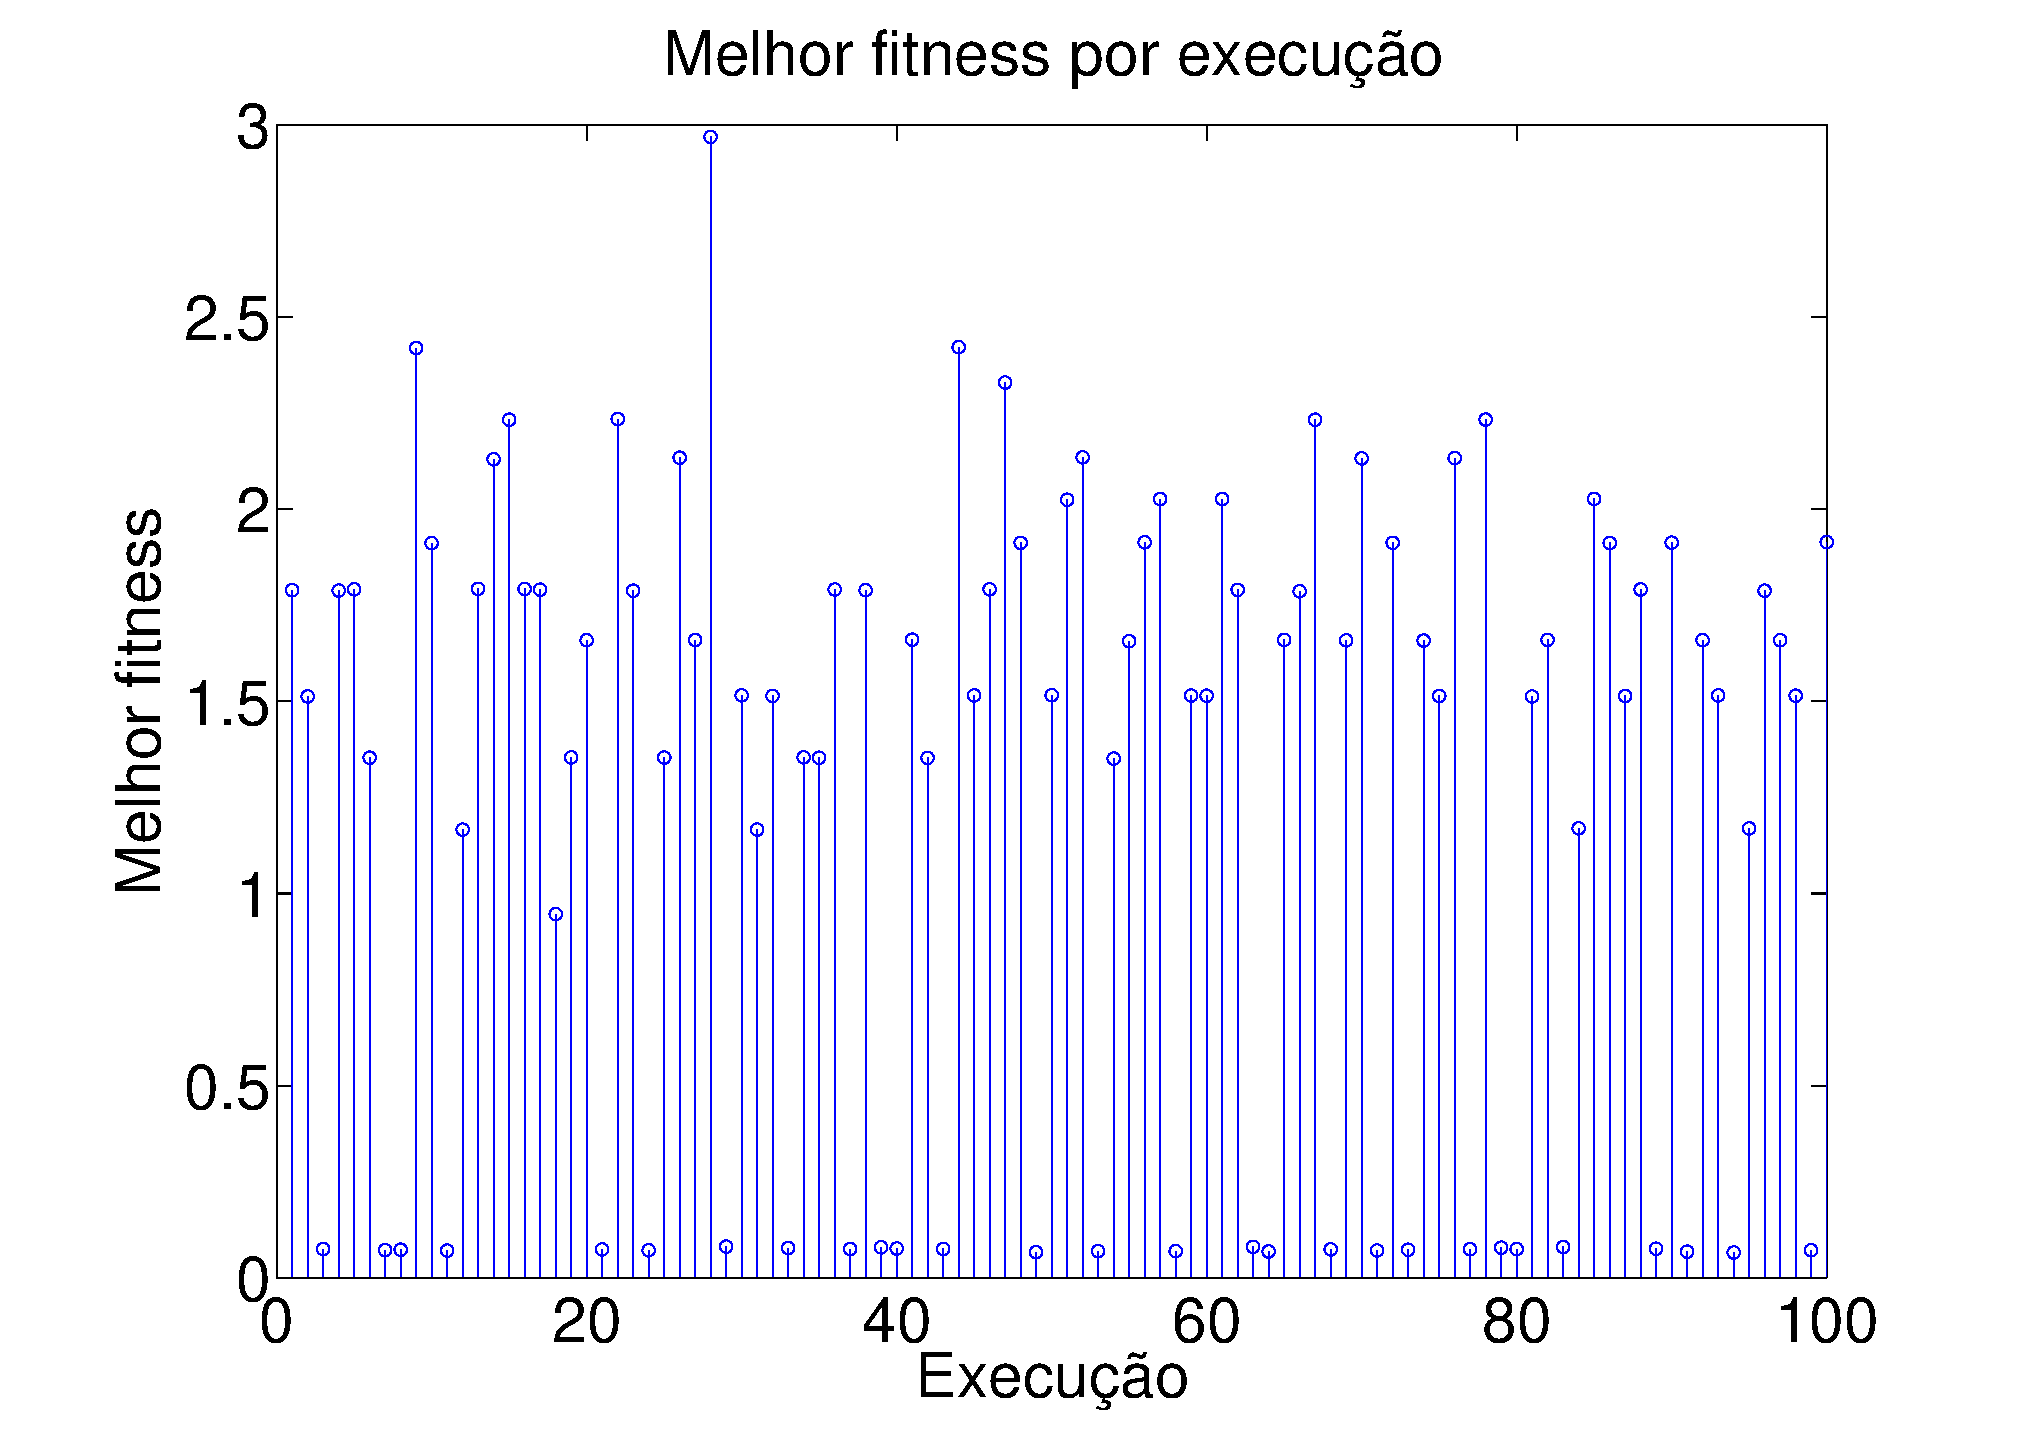
\includegraphics[width = \textwidth]{Q01_melhores_fitness}
	\caption{Gráfico das melhores fitness ao longo de 100 execuções do algoritmo}
	\label{melhores_fitness_q01}
\end{figure}
	
\begin{figure}[H]
	\centering
	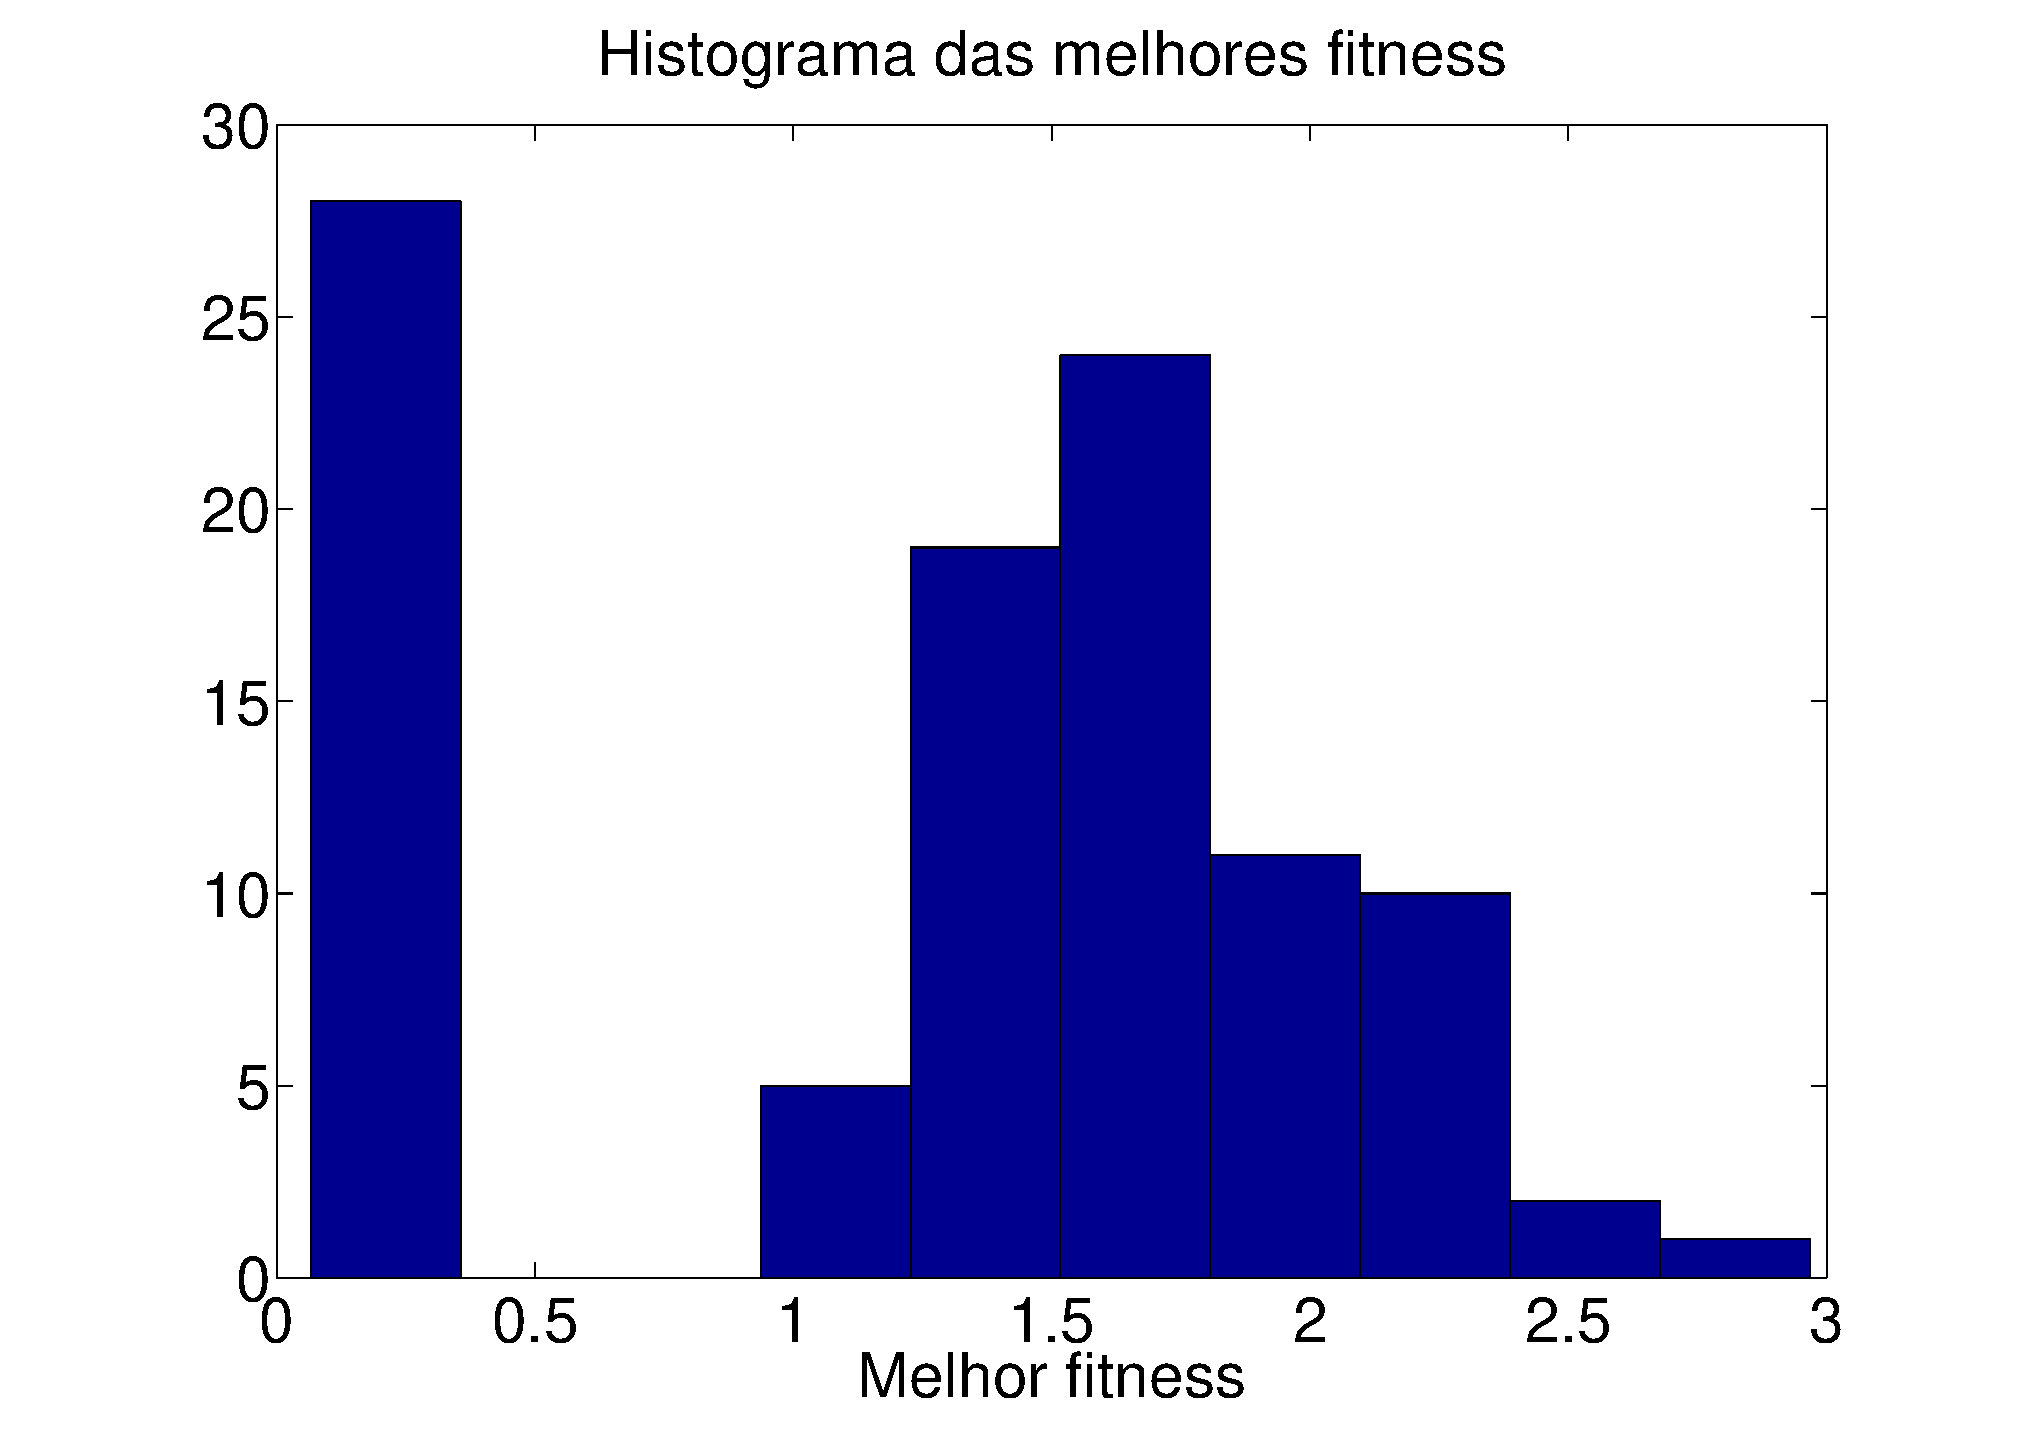
\includegraphics[width = \textwidth]{Q01_hist_melhores_fitness}
	\caption{Histograma das melhores fitness encontradas ao longo de 100 execuções do algoritmo}
	\label{hist_melhores_fitness_q01}
\end{figure}

\paragraph{} A Figura \ref{geracao_otima_q01} mostra as gerações em que as melhores soluções de cada execução apareceram pela primeira vez e a Figura \ref{hist_geracao_otima_q01} exibe seu histograma. A análise do histograma mostra que em grande parte das execuções, a melhor solução foi alcançada após muitas gerações terem sido consideradas (inclusive, próximas do limite imposto de 1000 gerações). O gráfico mostra que a quantidade de gerações mínima, necessária para se encontrar a melhor solução, foi de aproximadamente 600 (mais precisamente, 579). Em média, foram consideradas 841 gerações, com desvio padrão de 112. Considerando que nenhuma das soluções encontradas ficou abaixo do limiar estabelecido e que um número relativamente elevado de gerações foi necessário para se alcançar a melhor solução da execução (que não é a ótima), indica-se que um número maior de gerações deva ser considerado, na busca por solução, de modo a se tentar obter mais soluções próximas do mínimo buscado.\\

\begin{figure}[H]
	\centering
	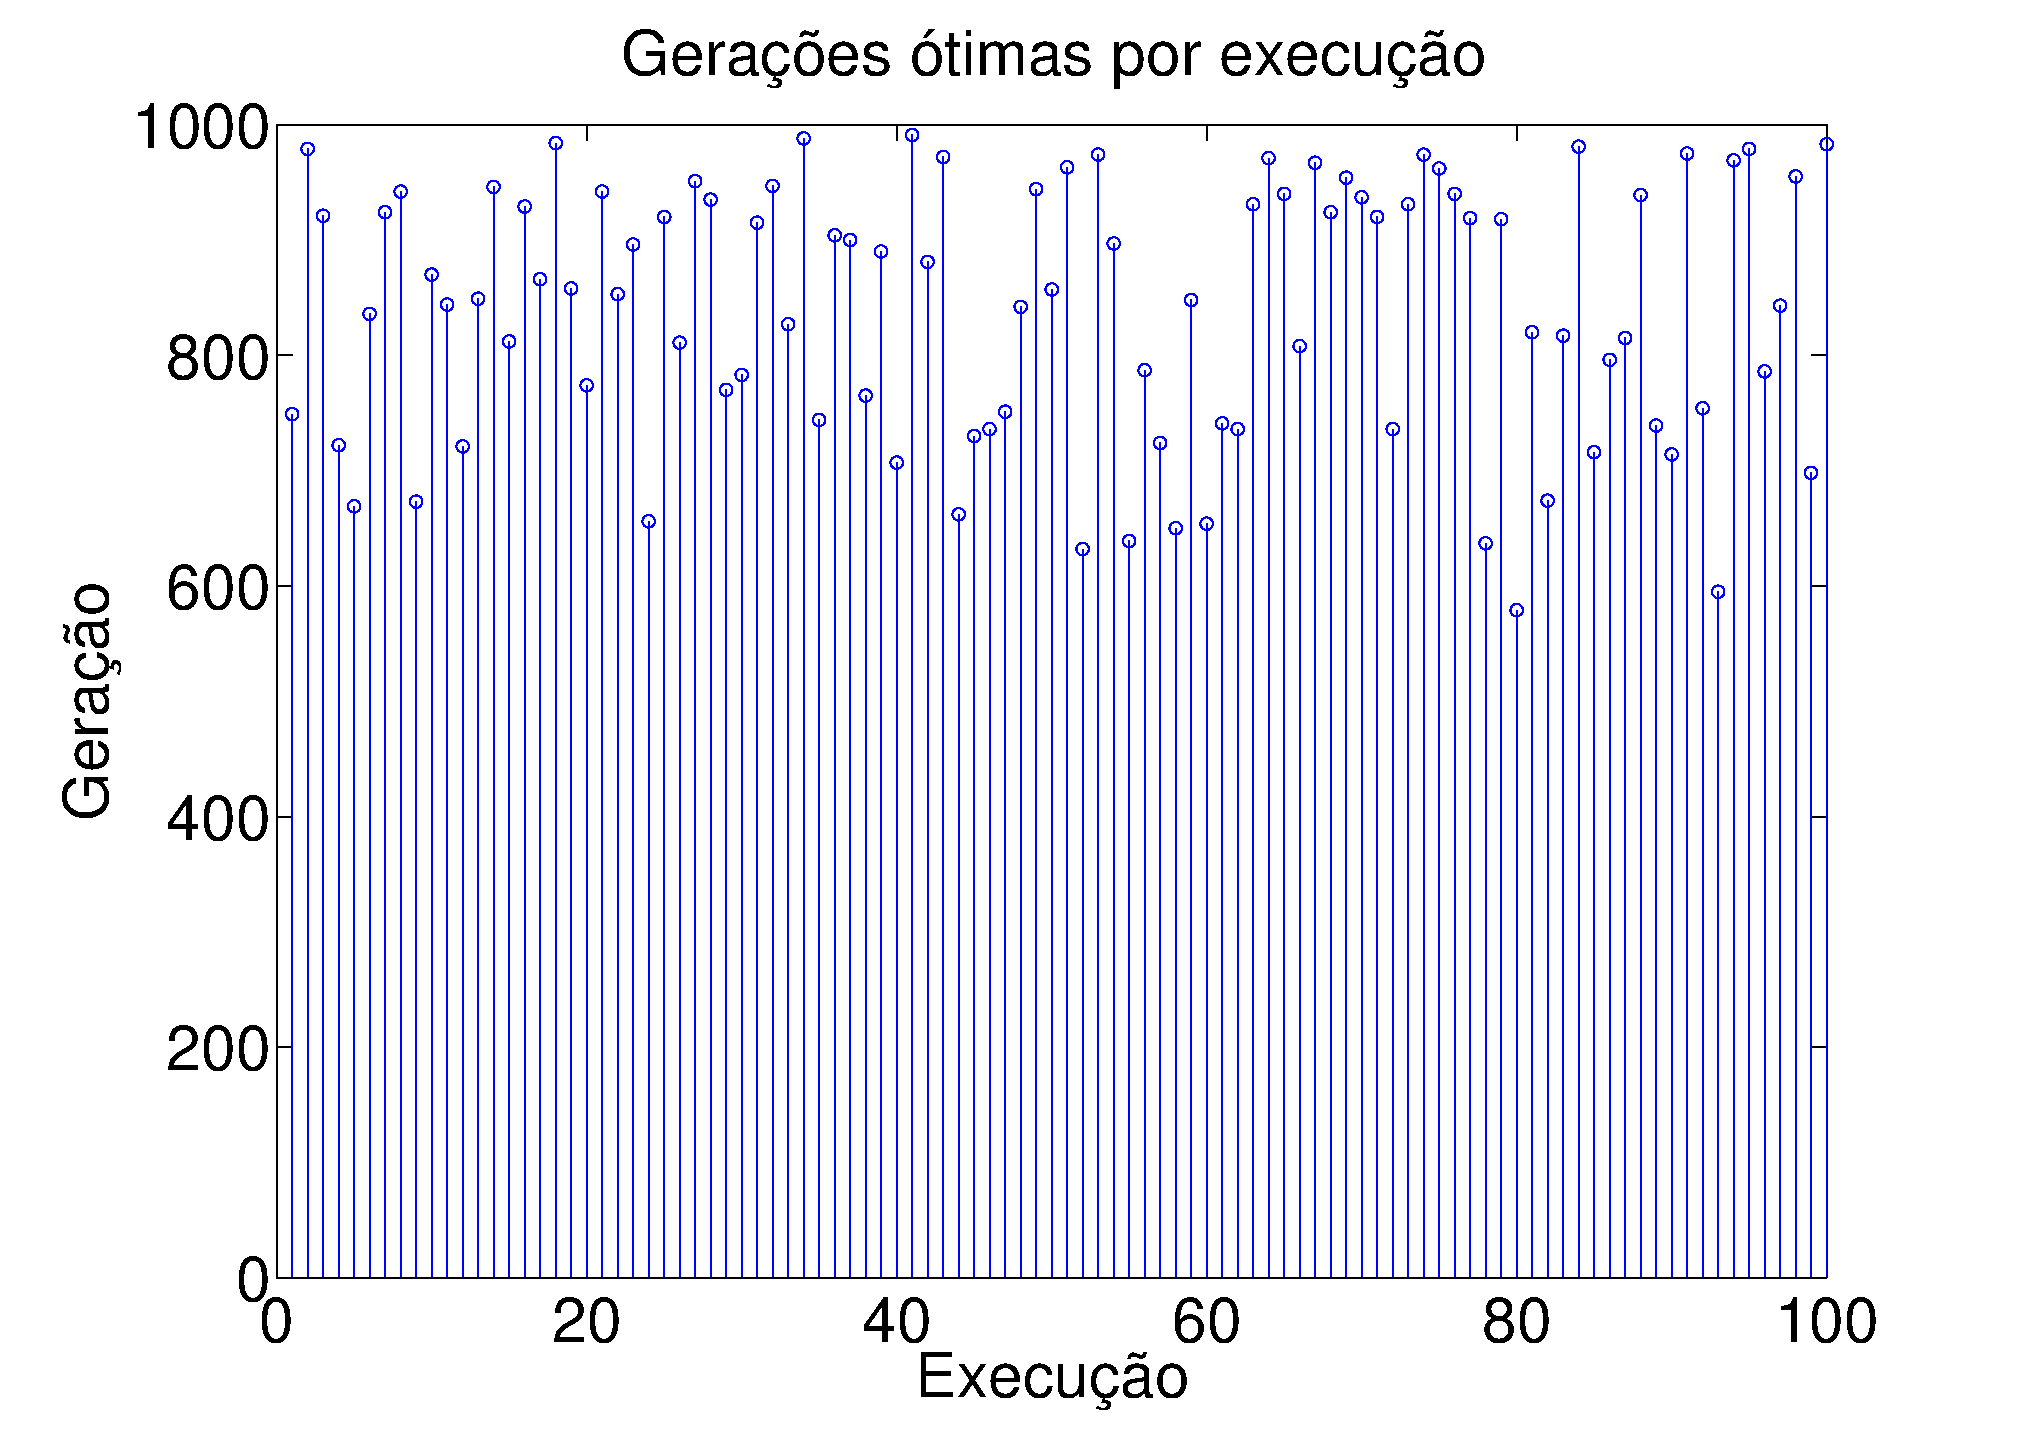
\includegraphics[width = \textwidth]{Q01_geracao_otima}
	\caption{Gráfico das gerações, nas quais as melhores soluções da execução em questão foram encontradas pela primeira vez}
	\label{geracao_otima_q01}
\end{figure}
	
\begin{figure}[H]
	\centering
	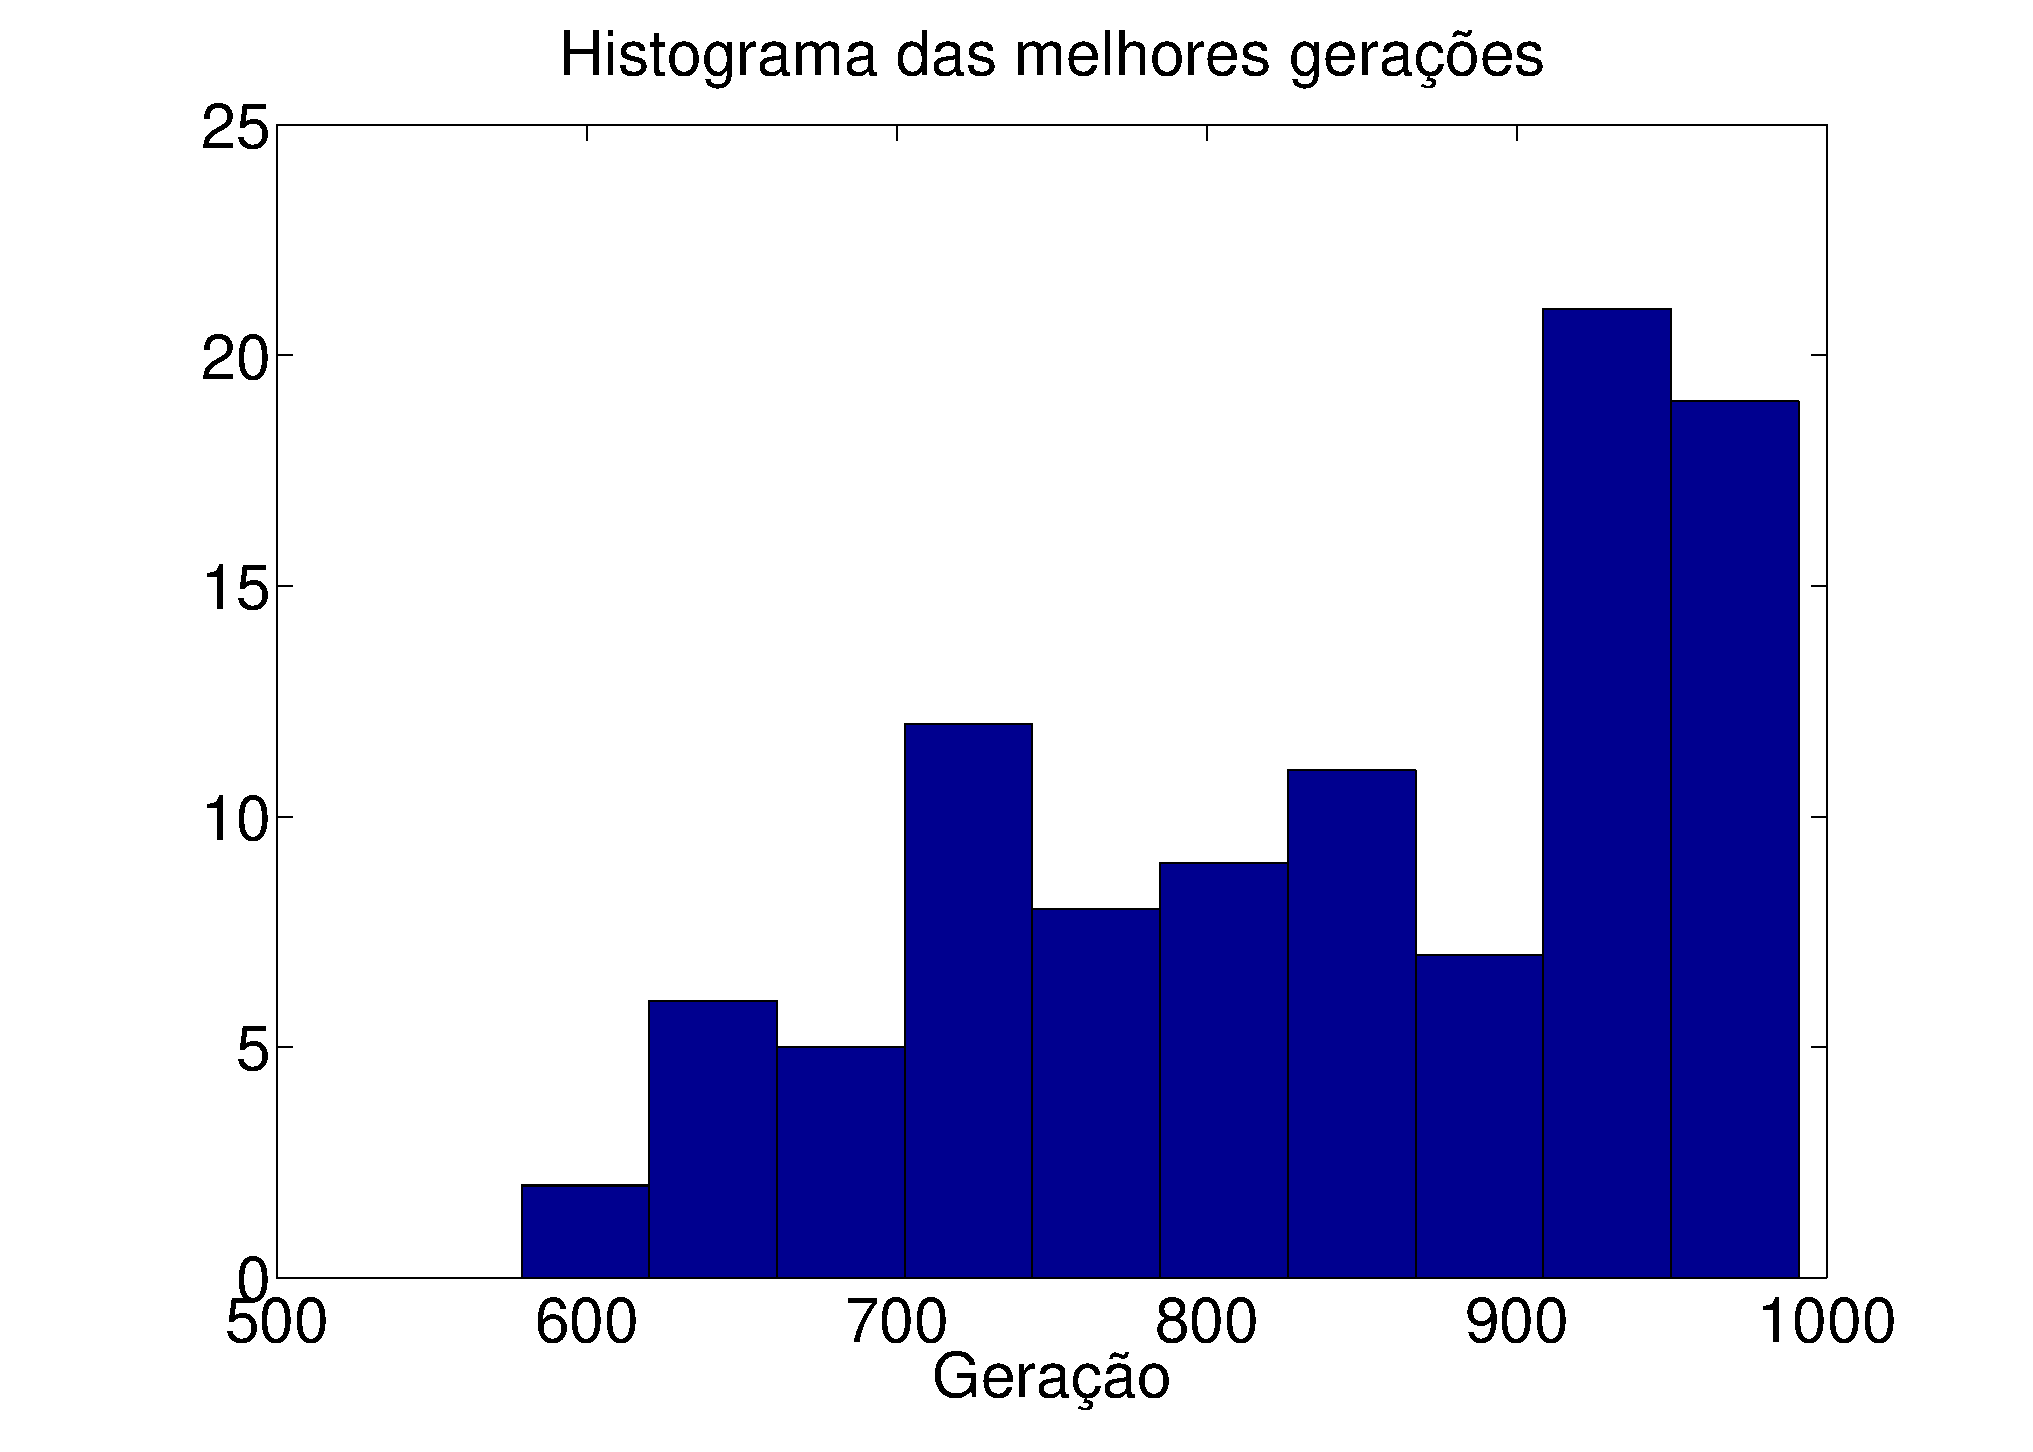
\includegraphics[width = \textwidth]{Q01_hist_geracao_otima}
	\caption{Histograma das gerações nas quais a melhor solução foi encontrada pela primeira vez ao longo das 100 execuções do algoritmo}
	\label{hist_geracao_otima_q01}
\end{figure}

\section*{Questão 2}

\textbf{\textit{Capítulo 14, Exercício 1}:}\\

\textbf{Consider using the number of generations as a measure to establish the speed of an EA. Compare the use of this measure with using the number of fitness evaluations.}\\

\paragraph{} Embora ambas sejam métricas válidas para se fazer uma avaliação da velocidade de execução de um algoritmo evolucionário, é preciso tomar cuidado em sua utilização na hora de se fazer comparações entre dois algoritmos. Considere, por exemplo, dois algoritmos, os quais utilizam como critério de parada a obtenção da solução ótima. O primeiro tem um processamento por geração mais lento (por conta, por exemplo, dos critérios de recombinação ou mutação selecionados), porém, em contrapartida, resulta em soluções bem próximas à ótima, ao passo que o segundo tem um processamento por geração mais rápido e resulta em soluções que se aproximam mais devagar da ótima. Devido à implementação dos algoritmos, supondo que ambos tenham alcançado a solução ótima, se o número de gerações fosse utilizado como critério para avaliar a velocidade de cada um, ter-se-ia a falsa impressão de que o primeiro é mais rápido que o segundo, por utilizar um número menor de gerações. Entretanto, na prática, por ter um processamento mais lento por geração, o tempo de execução de ambos pode ter sido semelhante, embora o segundo tenha precisado de mais gerações (compensado pelo fato de o processamento por geração ser mais rápido). Portanto, diversos outros fatores dos algoritmos podem impactar nessa medida e devem ser considerados.\\

\paragraph{} A utilização do número de avaliações da função de fitness tem a vantagem de retratar a capacidade do algoritmo em avaliar diferentes soluções para uma dada configuração do problema. Quanto mais rápido ele conseguir realizar cada avaliação, por exemplo, para um dado tamanho de população, mais soluções serão analisadas e, consequentemente, maiores são suas chances de encontrar a ótima. Por outro lado, caso a solução do problema não seja encontrada, essa métrica pode ser enganosa, tendo sido observado um alto número de avaliações, sugerindo uma alta velocidade, porém, não tendo êxito em resolver o problema. Nesse sentido, a utilização do número de gerações daria uma noção melhor do tempo de execução do algoritmo, já que um número elevado de gerações sugeriria uma demora do algoritmo em obter (caso alcance) a solução ótima. Entretanto, o número de gerações também tem a desvantagem de depender muito de outras etapas do algoritmo. Por exemplo, supondo que a inicialização da população tenha sido tal, que a solução ótima se encontrasse já na primeira geração. Essa métrica sugeriria uma velocidade do algoritmo muito distante da real, já que, circunstancialmente, outros fatores influenciaram essa convergência. Essas são algumas vantagens e desvantagens de cada uma dessas métricas. Vale lembrar que, por conta da estocacidade dos algoritmos genéticos, ambas as métricas só fazem sentido levando-se em conta suas propriedades estatísticas ao longo de diversas execuções independentes dos algoritmos a serem testados. Em todo caso, essas são algumas vantagens e desvantagens associadas a cada uma, as quais devem estar em mente, quando uma ou outra for escolhida como medida de desempenho. \\

\section*{Questão 3}

\textbf{\textit{Capítulo 8, Exercício 1}:}\\

\textbf{Give arguments why mutation strength (e.g., $p_m$ or $\sigma$) should be increased during a run. Give arguments why it should be decreased.}\\

\paragraph{} A adaptação da taxa e da magnitude do passo de mutação pode favorecer na busca de soluções, feita pelo algoritmo genético, melhorando seu desempenho, não só em relação ao tempo de execução do algoritmo (quanto tempo ele leva para encontrar uma solução boa), mas também em relação à qualidade das soluções encontradas. Com isso, cabe a pergunta de quando (e como) tais taxas devem variar. Sendo assim, analisa-se, primeiro, quando elas devem mudar.\\

\paragraph{} Aumentar esses parâmetros podem ser feitos, quando o resultado das mutações tem um efeito mais positivo do que degenerativo na população final, ou seja, a maioria dos indivíduos gerados por meio de mutação apresentam aptidões melhores do que os indivíduos anteriores. O argumento para tal é que se esse fato é observado, então, no espaço de soluções, os indivíduos da população atual encontram-se distantes das soluções ótimas (tanto global quanto locais). Sendo assim, aumentar o valor desses parâmetros, isto é, aumentar a taxa de mutação e/ou a magnitude do passo faz com que os indivíduos deixem essas regiões sub-ótimas mais rapidamente (analogamente, que se aproximem das regiões melhores mais rapidamente), evitando-se gastar muito tempo em regiões, nas quais as soluções estão longe das desejadas.\\

\paragraph{} Valores elevados desses parâmetros podem ter efeitos contrários, quando a população se situa próxima a um ótimo, que pode ser local ou global. Nesse caso, é interessante que tais valores sejam reduzidos, de forma a se realizar um ajuste mais fino dos indíviduos sobre a região do espaço de soluções em que se encontram, permitindo que a solução ótima seja, eventualmente, atingida. Estes são os casos, nos quais a solução ótima está próxima das soluções representadas pelos indivíduos em questão. Por um lado, a redução no valor de tais parâmetros é válida, pois, supondo que a população está convergindo para a solução ótima, mutações frequentes ou passos largos tenderiam a gerar mais indivíduos menos aptos do que indivíduos mais aptos, o que não é desejado. Por outro lado, caso não se esteja no ótimo global, o algoritmo ficará preso na região do ótimo local. Sendo assim, ainda que a redução do valor dos parâmetros de mutação seja benéfica, quando a mutação rende, em sua maioria, indivíduos menos aptos, é preciso garantir uma certa diversidade da população, de modo a permitir que o algoritmo escape de ótimos locais (e possa, eventualmente, atingir a região do ótimo global). Garantindo essa diversidade, pode-se aplicar a regra proposta para aumento/redução nos valores dos parâmetros de mutação: maiores, para indivíduos longe da região ótima, e menores, para indivíduos próximos da região ótima.\\

\section*{Questão 4}

\textbf{Considere o problema básico de \textit{clustering} em que colunas $\mathbf{x}(n), n = 1,...,N$ da matriz de dados $\mathbf{X}$ devem ser representadas, de forma aproximada, pelas colunas $\mathbf{y}(k), k = 1,...,K$ do dicionário $\mathbf{Y}$ de forma que seja minimizado o erro médio quadrático:}\\

\begin{equation*}
D = \frac{1}{N} \sum_{n = 1}^{N}||\mathbf{x}(n) - \mathbf{y}(k(n))||^2
\end{equation*}\\

\textbf{onde $k(n) = argmin_i||\mathbf{x}(n) - \mathbf{y(i)}||$. Utilizando pseudo-código, escreva um algoritmo genético simples que, operando sobre uma população de dicionários $\mathbf{Y}$, leve à obtenção de uma solução $\mathbf{Y^*}$ localmente ótima para este problema. Defina todos os parâmetros que você julgar necessários.}\\

\paragraph{}

\end{document}